\documentclass{article} % For LaTeX2e
\usepackage{nips14submit_e,times}
\usepackage{hyperref}
\usepackage{cite}
\usepackage{url}
\usepackage{graphicx}
\usepackage{float}
\usepackage{amsmath}
\usepackage{amssymb}

\title{Mid-Term Paper : \\Freesound General-Purpose Audio Tagging Challenge}


\author{
Sarah Gross \\
Master of Advanced Computing \thanks{\url{http://ac.cs.tsinghua.edu.cn/}}\\
Tsinghua University\\
\texttt{leihy17@mails.tsinghua.edu.cn} \\
\And
Usama Zafar\\
Master of Advanced Computing\\
Tsinghua University\\
\texttt{zafaru10@mails.tsinghua.edu.cn} \\
}


\newcommand{\fix}{\marginpar{FIX}}
\newcommand{\new}{\marginpar{NEW}}

%\nipsfinalcopy % Uncomment for camera-ready version

\begin{document}


\maketitle

\begin{abstract}
	Sound tagging has been studied for at least a couple of decades now. Among the different types of sounds the most prevalent research areas have been music, speech and enviromental sounds. Some sounds are distinct and instantly recognizable, like a baby's laugh or the strum of a guitar. Other sounds aren't clear and are difficult to pinpoint, or are drowned in a mix of sounds that are difficult to identify individually.\\
	\newline
    Partly because of the vastness of sounds we experience, no reliable automatic general-purpose audio tagging systems exist. Currently, a lot of manual effort is required for tasks like annotating sound collections and providing captions for non-speech events in audiovisual content.\\
	\newline
    This project's goal is to be able to recognize an increased number of sound events of very diverse nature, and to leverage subsets of training data featuring annotations of varying reliability.
\end{abstract}

\section*{Introduction}
    Our life is surrounded by various sounds: speech, music, animal call, aircraft, traffic, even the sound of typing words, clicking the mouse, etc. Sounds can be roughly grouped into three clusters: human voice, artificial sound, and non-artificial/natural sound.\\
    \newline
    Human voice refers to sounds created by people physically such as speech, cough, and singing. Artificial sounds refer to sounds created by human activities such as traffic, aircraft, and music. Non- artificial sounds include sounds created by nature such as wind, rain, land animal, insects and marine life.\\
    \newline
    These sounds make the world exclamatory and colourful. All these sounds carry information and have their own characteristics. In order to categorise different kinds of sounds and study them separately, tagging is introduced into the area of sound analysis. The act of tagging, in this context refers to the action of adding text based on metadata and annotations to specific non-textual information and data.\\
    \newline
    Initially, people classified and documented all information manually. If you close your eyes, could you tell the difference between the sound of a chainsaw and a blender? Probably not. With the development of machine technology, especially the computer science, people started to study new ways of automatic tagging, not only due to its accuracy but also due to its performance. A lot of classification work has been solved efficiently for music, speech and environmental sounds.\\
    \newline
    However, despite the good performance, these automatic tagging machines still need information from the metadata of targets. The metadata is collected manually in several ways. Besides one model suited for tagging one classification of sounds might not be suited for the other classes. And often times than not it is the case that sounds are not distinguished into their respective classes. This is where machine learning comes into play, in cases such as these, there is a need for general purpose tagging systems.


\section{Dataset}
	\subsection{About the dataset}
		Freesound Dataset Kaggle 2018 (or FSDKaggle2018 for short) is an audio dataset containing 18,873 .wav files annotated with 41 labels from Google's AudioSet Ontology \cite{cite1}:\\

			"Acoustic\_guitar", "Applause", "Bark", "Bass\_drum", "Burping\_or\_eructation", "Bus", "Cello", "Chime", "Clarinet", "Computer\_keyboard", "Cough", "Cowbell", "Double\_bass", "Drawer\_open\_or\_close", "Electric\_piano", "Fart", "Finger\_snapping", "Fireworks", "Flute", "Glockenspiel", "Gong", "Gunshot\_or\_gunfire", "Harmonica", "Hi-hat", "Keys\_jangling", "Knock", "Laughter", "Meow", "Microwave\_oven", "Oboe", "Saxophone", "Scissors", "Shatter", "Snare\_drum", "Squeak", "Tambourine", "Tearing", "Telephone", "Trumpet", "Violin\_or\_fiddle", "Writing"\\
			\newline

		More information is accessible on 
		\begin{center} 
		\url{https://www.kaggle.com/c/freesound-audio-tagging/data}
		\end{center}

		We use a first subset au audio files \emph{audio\_train} to train our model, and a second subset \emph{audio\_test} for evaluating our model.\\
		The labels for train dataset are wirtten in train.csv. It contains the following information:
		\begin{itemize}
		    \item fname: the file name
		    \item label: the audio classification label (ground truth
		    \item manually\_verified: Boolean (1 or 0) flag to indicate whether or not that annotation has been manually verified.
		\end{itemize}

	\subsection{Dataset analysis}
		We first plotted the distribution of samples per label \ref{fig:category_distribution}.
		\begin{figure}[H]
		  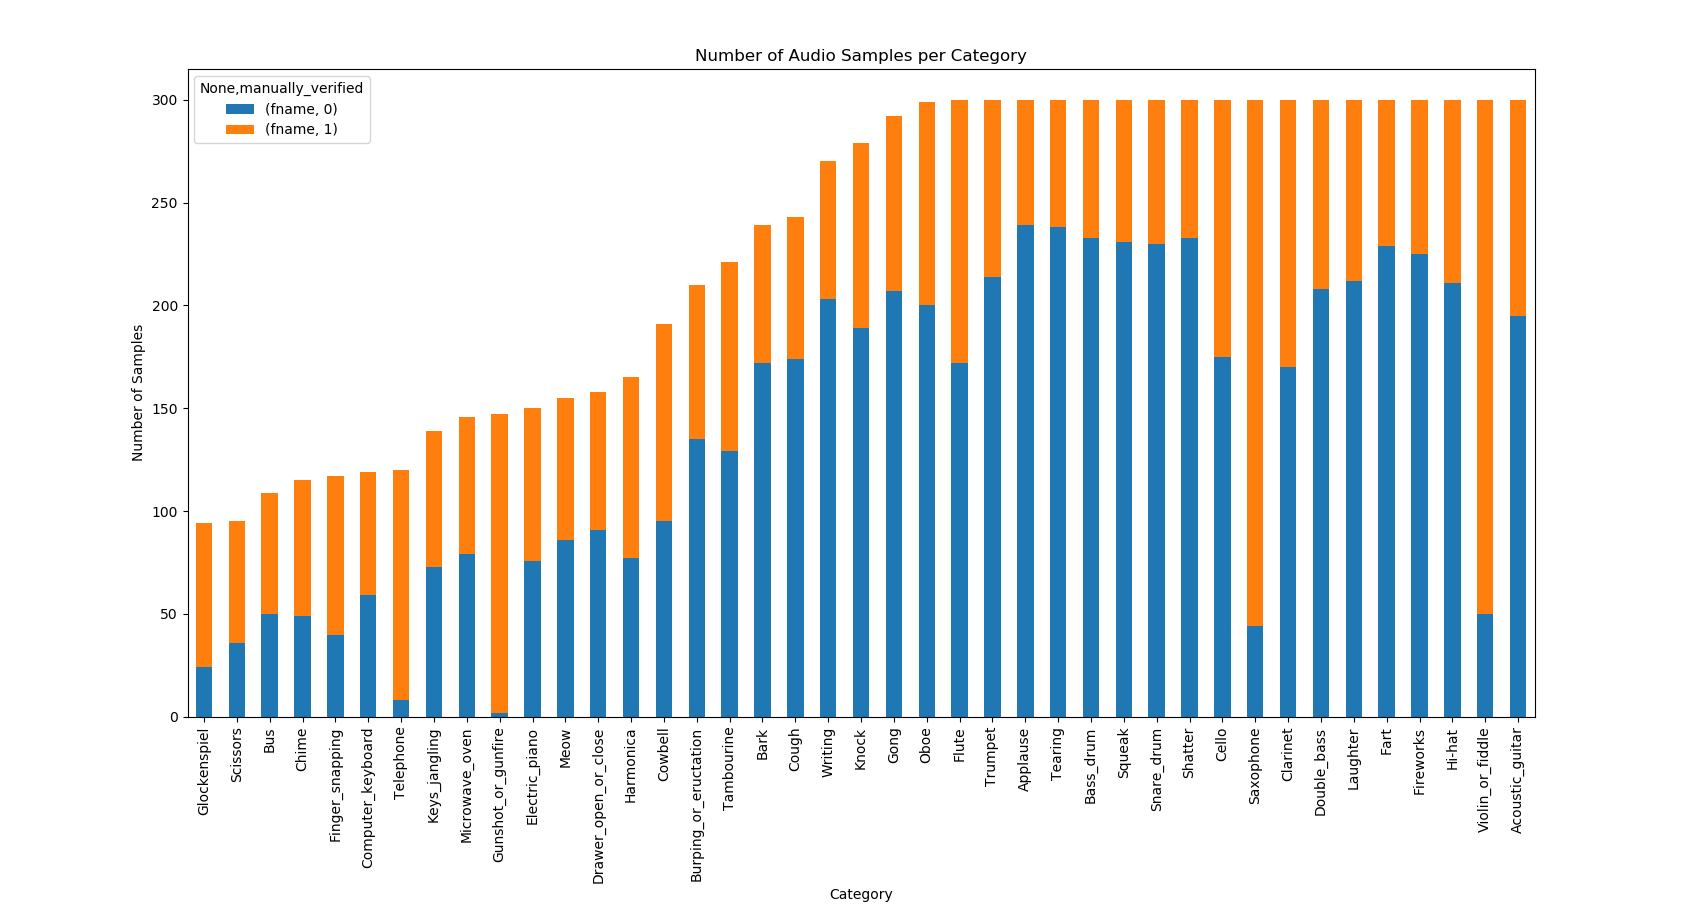
\includegraphics[width=\linewidth]{category_distribution.png}
		  \caption{Distribution of samples per category}
		  \label{fig:category_distribution}
		\end{figure}
		We notice two phenomena :
		\begin{itemize}
		    \item There is a highly unequal distribution of samples over the labels
		    \item The number of verified data varies over the labels
		\end{itemize}

		We can visualize the difference between the samples by using some useful tools from the python package for music and audio analysis LibROSA\footnote{\url{http://librosa.github.io/librosa/}}. We picked randomly 4 samples \emph{Oboe, Fireworks, Cello, Harmonica} and plot various graphs \ref{fig:graphs} :

		\begin{itemize}
		    \item The Waveplot
		    \item The Spectrogram
		    \item The Log Spectrogram
		\end{itemize}


		\begin{figure}[H]
		  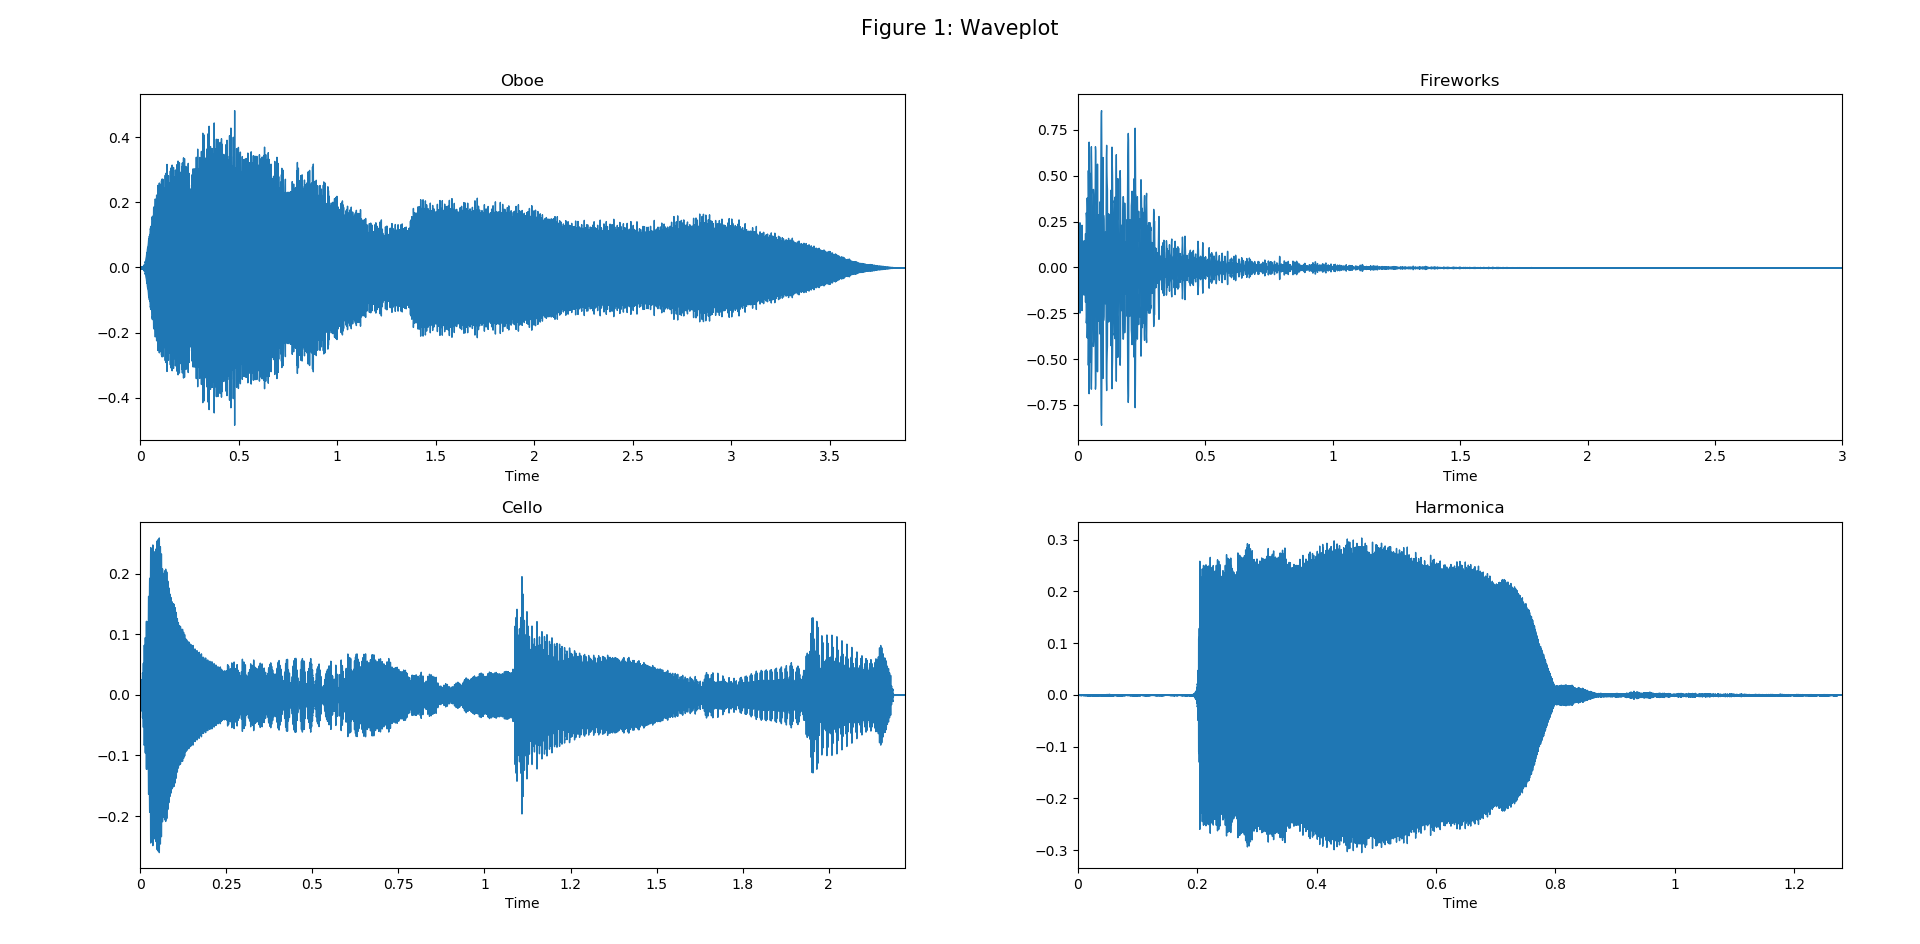
\includegraphics[width=\linewidth]{waveplot.png}
	  	\end{figure}
	  	\begin{figure}[H]
		  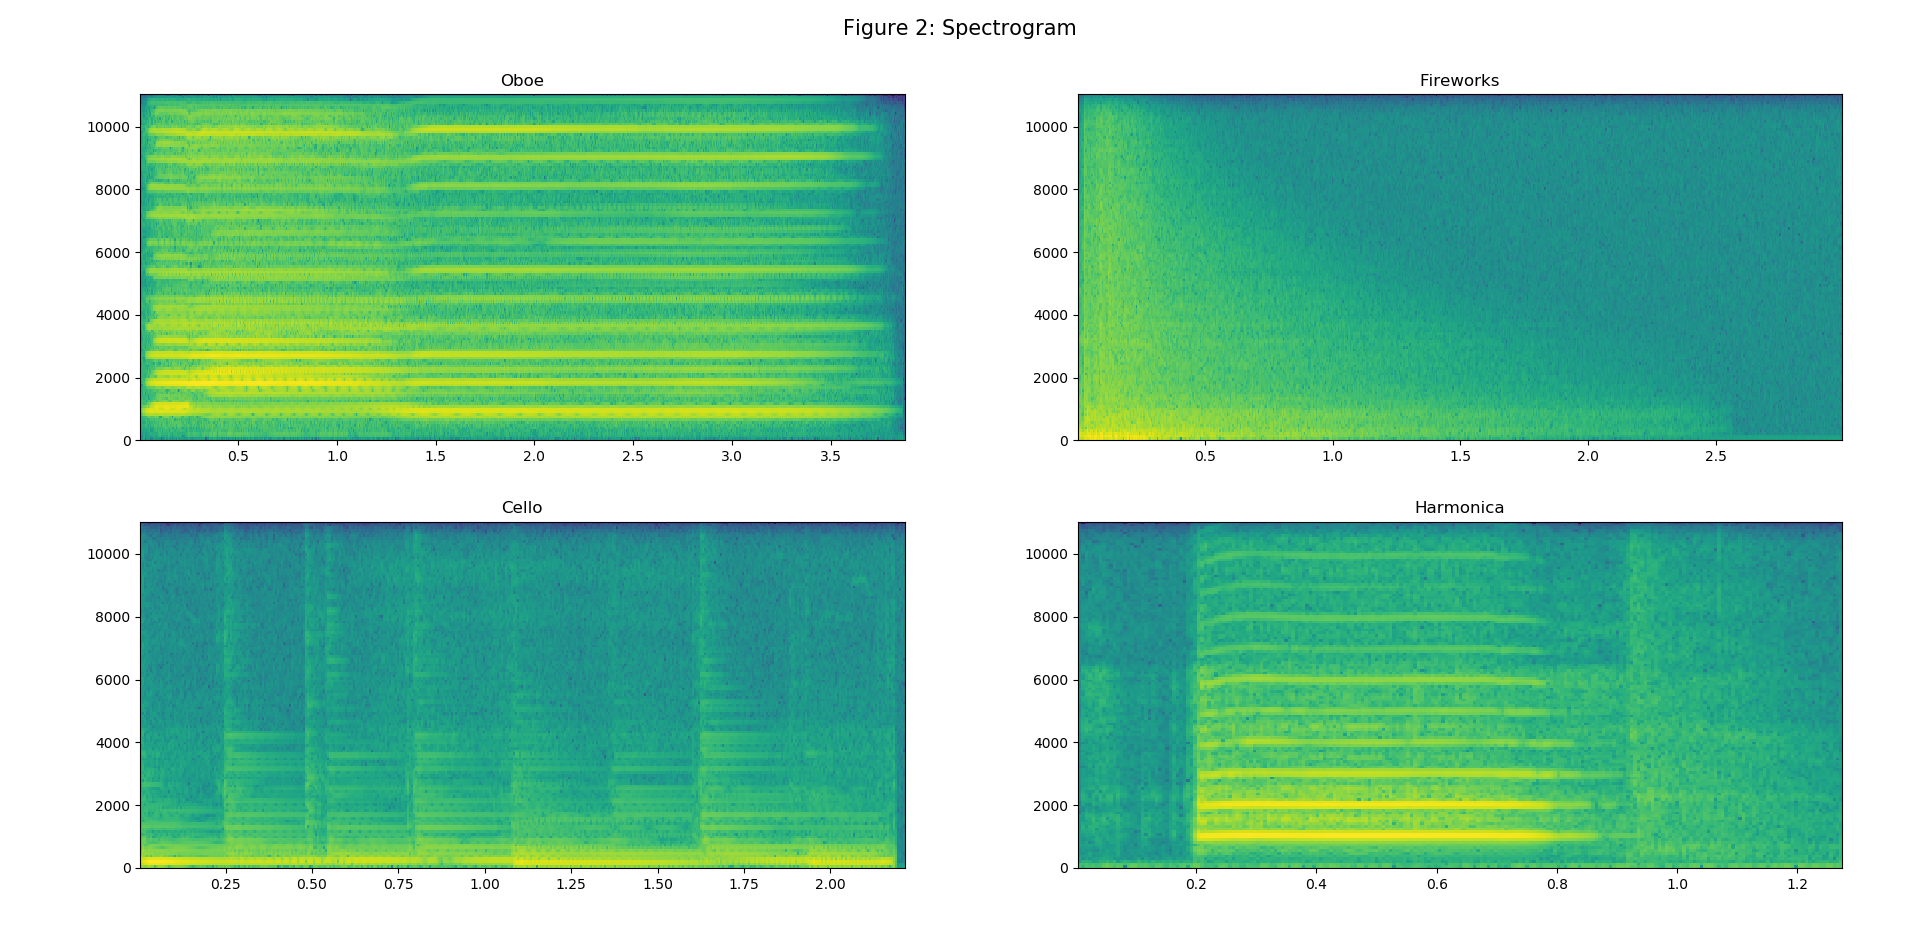
\includegraphics[width=\linewidth]{spectrogram.png}
	  	\end{figure}
	  	\begin{figure}[H]
		  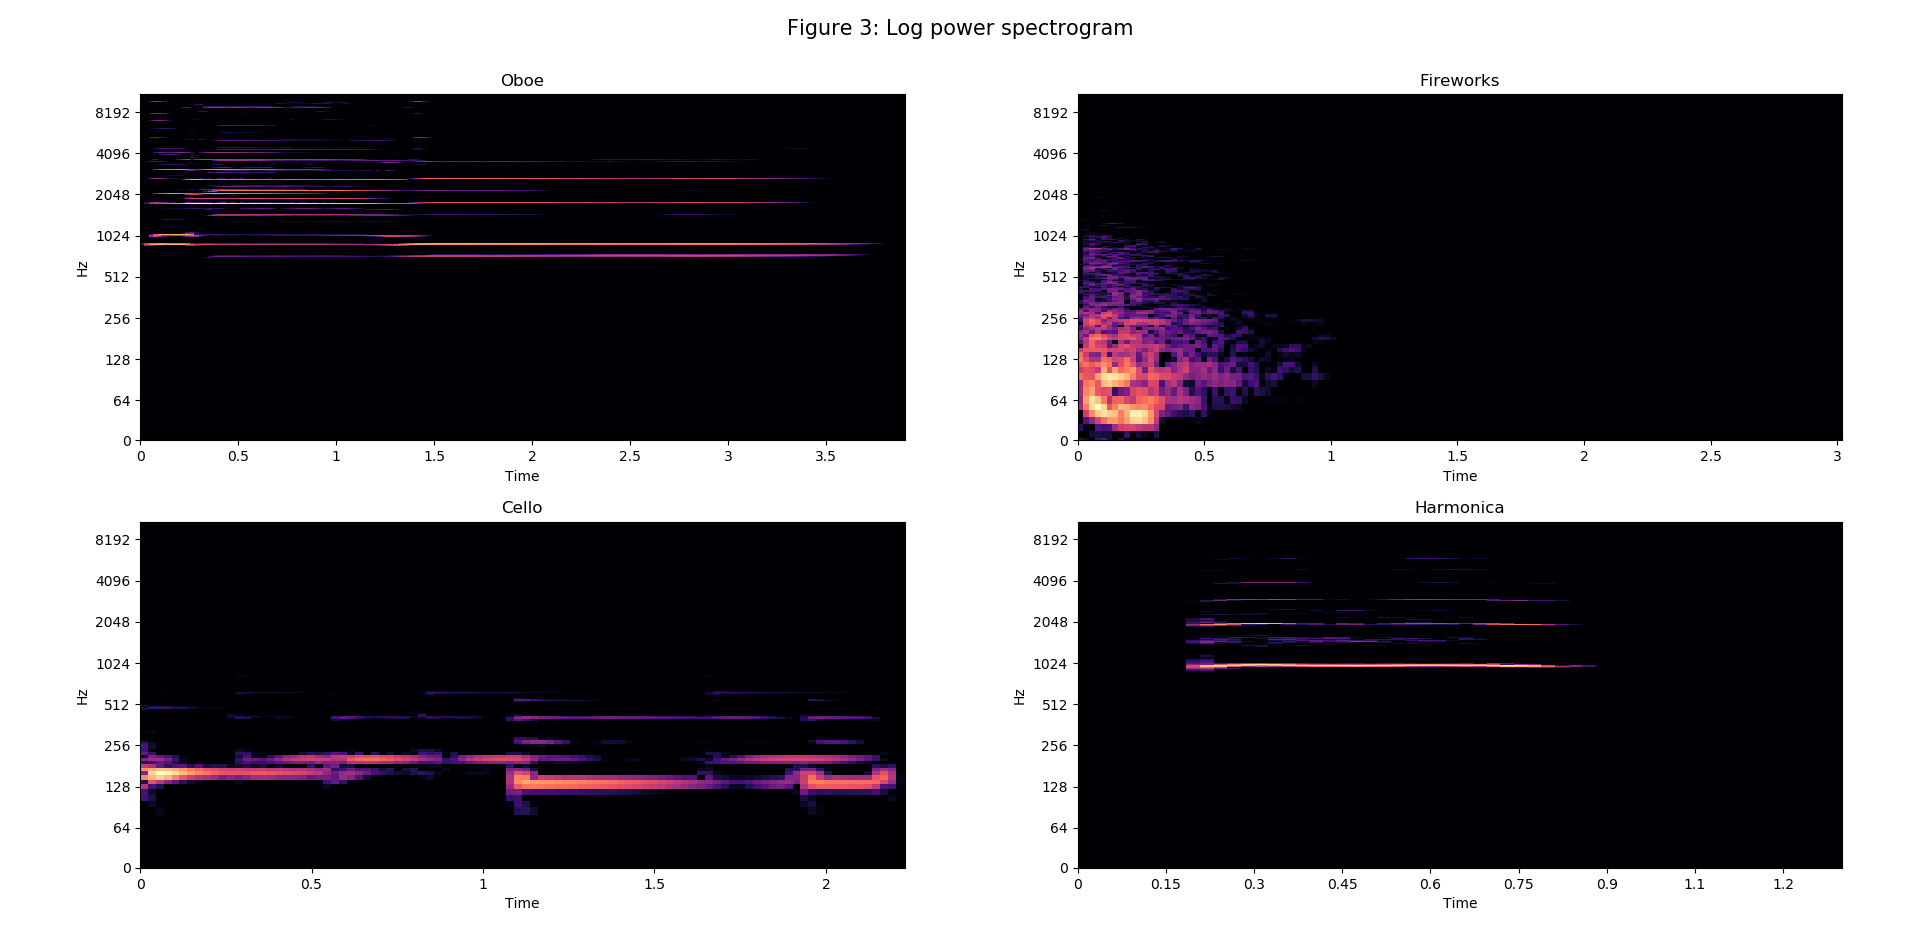
\includegraphics[width=\linewidth]{logspectrogram.png}
		  \caption{Useful tools for analysis sounds provided by Librosa}
		  \label{fig:graphs}
		\end{figure}

		We see that we get very different kinds of outputs and there is no way to visually guess which graphs belong to which sound.
		Usually, in sound analysis, the raw samples are very complex and it is difficult to get valuable information directly from them, especially if they contain noise.
		This is why we won't use the raw samples but extract some features from the sample which will, in contrary, give significant information that will help us make the classification.

\section{Feature Extraction}
    In machine learning, pattern recognition and image processing, feature extraction is a process to extracting a subset of features to be used for training. Feature extraction can be carried out for any number of reasons some of which are (but not limited to), to reduce the amount of resources required to describe large set of data, remove redundancy, get best set of features etc.\\\\
    In our case with audio data we use feature extraction to get different audio related features that can be used to train our model. Simply using time-frequency series as an input for learning is not optimal and hence we need some better approach to get otpimal features. This brings us to Mel Frequency Cepstral Coefficient (MFCC). Another reason for this preprocessing on audio data is because we want to saturate the actual sound/intended sound from any auxilary sounds present in the audio files. Feature extraction also helps us minimize effects of background noise etc.\\\\
	\subsection{Mel Frequency Cepstal Coefficients}
		Mel Frequency Cepstral Coefficents (MFCCs) are a feature widely used in automatic speech and speaker recognition. They were introduced by Davis and Mermelstein in the 1980's, and have been state-of-the-art ever since. Prior to the introduction of MFCCs, Linear Prediction Coefficients (LPCs) and Linear Prediction Cepstral Coefficients (LPCCs) and were the main feature type for automatic speech recognition (ASR), especially with HMM classifiers.\\\\
		In the next section we will briefly look at the steps involved in extracting mfcc features.
%		Why use feature extraction ? Use mathematics \url{http://practicalcryptography.com/miscellaneous/machine-learning/guide-mel-frequency-cepstral-coefficients-mfccs/}
	\subsection{Mel Frequency - Extraction Process}
	Typical steps involved with extracting mfcc features of an audio signal are as follows:
    \begin{enumerate}
        \item Frame the signal into short frames
        \item For each frame calculate the periodogram estimates of the power spectrum
        \item Apply the mel filterbank to the power spectra, sum the energy in each filter.
        \item Take the logarithm of all filterbank energies.
        \item Take the DCT of the log filterbank energies.
        \item Keep DCT coefficients 2-13, discard the rest.
    \end{enumerate}
    \subsection{Extraction Process - Theory}
	In this section we look in detail at the theory behind each of the step involved in mfcc extraction process.
	\begin{enumerate}
		\item An audio signal is constantly changing, so to simplify things we assume that on short time scales the audio signal doesn't change much (when we say it doesn't change, we mean statistically i.e. statistically stationary, obviously the samples are constantly changing on even short time scales). This is why we frame the signal into 20-40ms frames. If the frame is much shorter we don't have enough samples to get a reliable spectral estimate, if it is longer the signal changes too much throughout the frame. 25ms is standard. In out case, we have a sample rate of 44.1 kHz which gives $N = 0.025 \times 44100 = 1102.5$ samples in case of 25ms sampling.\\\\
			The next steps are applied to every single frame, one set of 12 MFCC coefficients is extracted for each frame.\\ We call our time domain signal $s(n)$. Once it is framed we have $s_i(n)$ where n ranges over 1 to $N$ samples and $i$ ranges over the number of frames. When we calculate the complex DFT, we get $S_i(k)$ - where the $i$ denotes the frame number corresponding to the time-domain frame. $P_i(k)$ is then the power spectrum of frame $i$.
		\item We calculate the power spectrum of each frame, to modelize the way human ear transmits information to the brain.\\
		We first make a Discret Fourier Transform of the frame:\\
		$$S_i(k) = \displaystyle\sum_{n=1}^N s_i(n)h(n)e^{j2\pi kn /N}, \quad 1 \leq k \leq K$$
		where $h(n)$ is an $N$ sample long analysis window (e.g. hamming window), and $K$ is the length of the DFT.\\
		Then we get periodogram-based power spectral estimate for the speech frame $S_i(n)$ by taking the absolute value of the complex fourier transform and square the result:\\
		$$P_i(k) = \frac{1}{N} |S_i(k)|^2$$

		\item We compute the Mel-spaced filterbank. This is a set of 20-40 (26 is standard) triangular filters that we apply to the periodogram power spectral estimate from step 2. Each vector is mostly zeros, but is non-zero for a certain section of the spectrum. \\
		For instance, the first filterbank will start at the first point, reach its peak at the second point, then return to zero at the 3rd point. The second filterbank will start at the 2nd point, reach its max at the 3rd, then be zero at the 4th etc. A formula for calculating these is as follows:\\
		\[H_m(k) =
			\begin{cases}
				0 \quad k < f(m-1) \\\\
				\frac{k-f(m-1)}{f(m)-f(m-1)} \quad f(m-1) \leq k \leq f(m) \\\\
				\frac{f(m+1)-k}{f(m+1)-f(m)} \quad f(m) \leq k \leq f(m+1) \\\\
				0 \quad k > f(m+1) \\
			\end{cases}
		\]
		where $M$ is the number of filters we want, and $f()$ is the list of $M+2$ Mel-spaced frequencies.\\
		We convert frequency from Hz to Mel using the formula :\\
		$$ M(f) = 1125 ln(1 + f/700) $$
		Then, to calculate filterbank energies we multiply each filterbank with the power spectrum, then add up the coefficents as described in the following figure \ref{fig:melfilterbank}:
		\begin{figure}[H]
		  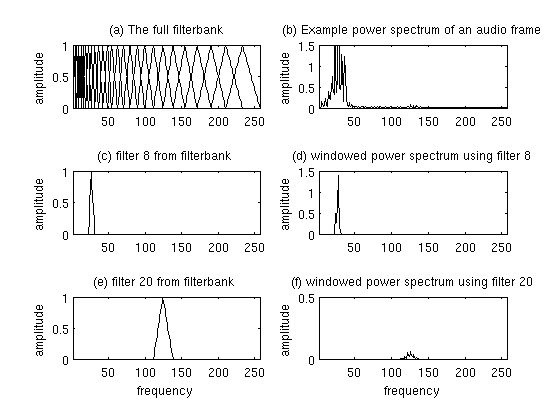
\includegraphics[width=\linewidth]{mel_filterbank_example}
		  \caption{Plot of Mel Filterbank and windowed power spectrum}
		  \label{fig:melfilterbank}
	  	\end{figure}

	  	\item Take the log of each of the 26 energies from step 3. This leaves us with 26 log filterbank energies.

		\item Take the Discrete Cosine Transform (DCT) of the 26 log filterbank energies to give 26 cepstral coefficents. For ASR, only the lower 12-13 of the 26 coefficients are kept.

	\end{enumerate}
	The resulting features (12 numbers for each frame) are called Mel Frequency Cepstral Coefficients.

	\subsection{Implementation}
		We used the librabry LibROSA, which appears in many works related to sound classification such as K. Pizcack's \cite{cite2}.\\
		This makes it extremely easy to extract the features which we will use for our classification problem.

		\begin{enumerate}
			\item First, we get the \verb+.wav+ file in a raw format and its sample rate using \verb+librosa.load+. We use the parameter \verb+res_type='kaiser_fast+ which makes loading faster.
			\item We extract each feature by applying the dedicated Librosa functions on the raw sample and passing as parameter its sampling rate.
		\end{enumerate}
		Here are some examples of the output of MFCC using Librosa \ref{fig:mfccgraph}.
		\begin{figure}[H]
		  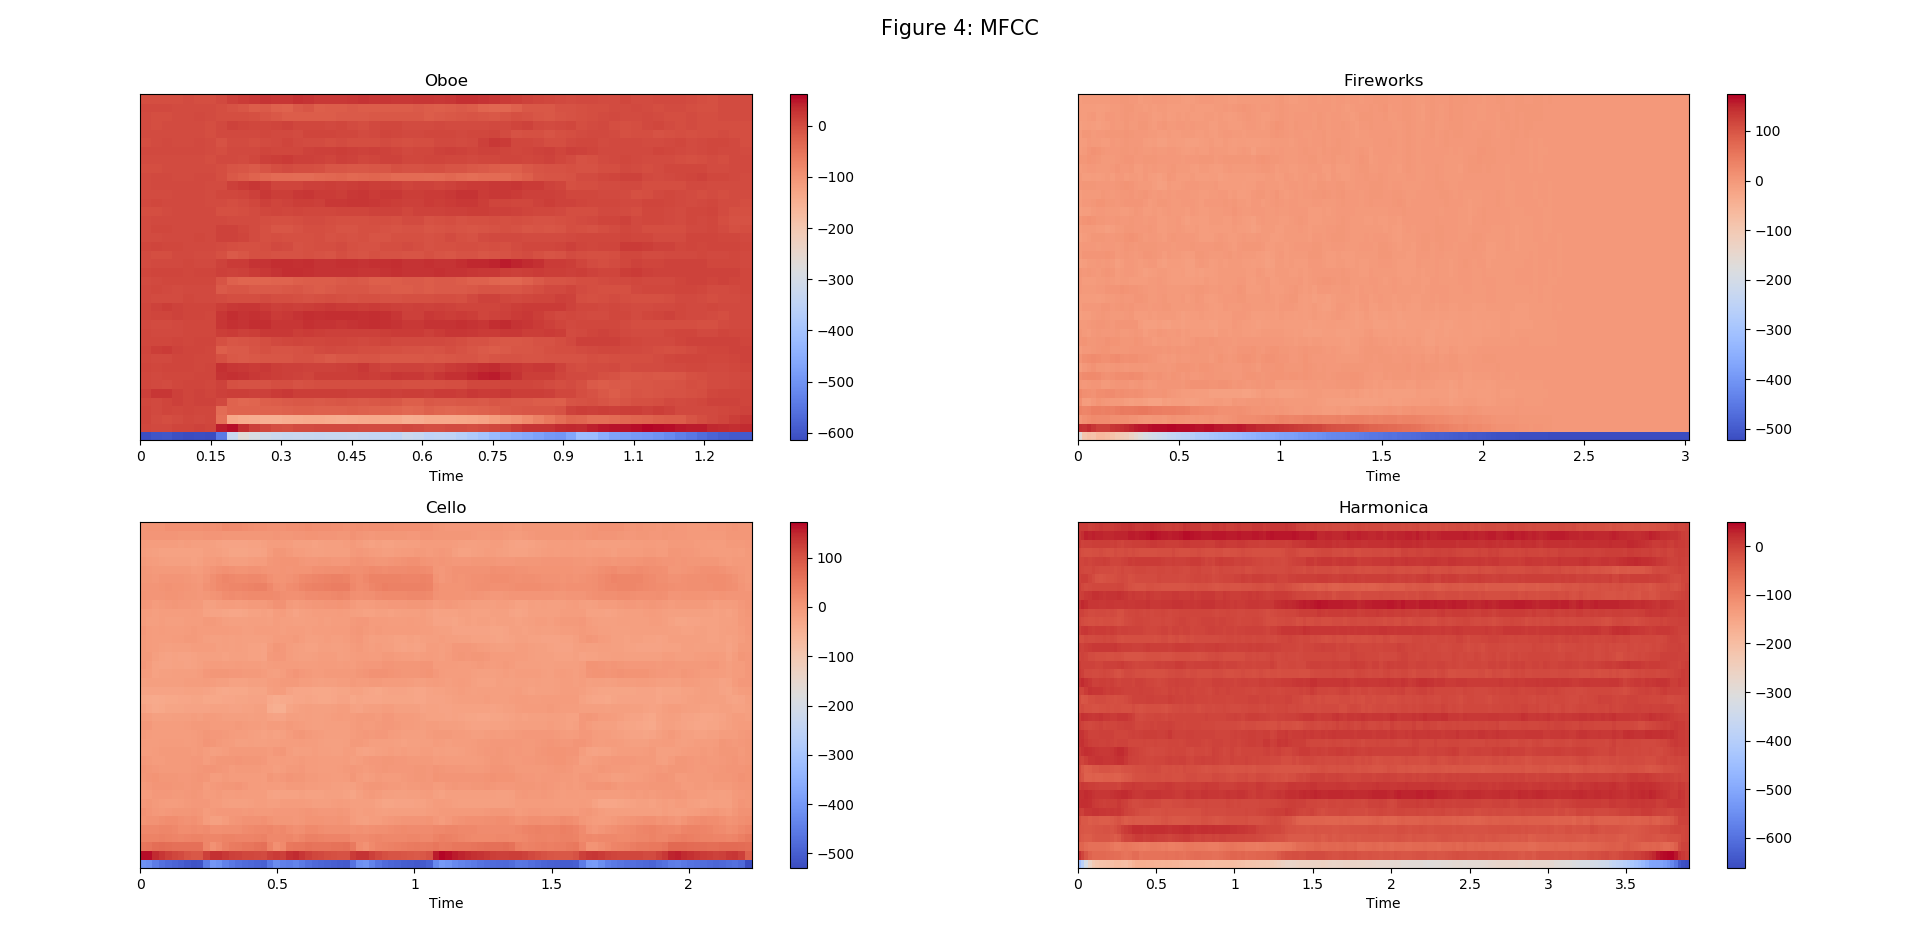
\includegraphics[width=\linewidth]{mfcc.png}
		  \caption{Mel Frequency Cepstral Coefficients}
		  \label{fig:mfccgraph}
		\end{figure}

\section{A Simple Neural Network}
		In our project proposal, we first proposed using Hidden Markov Model algorithm to classifiy the sounds.\\
		This choice was made with very little knowledge of this technique, because a few papers using it obtained good results \cite{cite3} \cite{cite4}. However after extensive research of the inner functionning of HMMs, we understood why many other papers of our survey disapproved using this algorithm \cite{cite5} \cite{cite6}. HMM's idea is to start from a known final state, and try to guess which sequence of actions was followed in order to get to that result. This path, or sequence of actions, is unknown hence the adjective \emph{hidden}. HMM are therefore very useful in cases there is an actual path to find, for instance in board games or speech recognition : in the latter case, the path consists of \emph{each word} spoken in the sentence.\\
		\newline
		However, in our case, we don't want to extract and analyse every little part that consists our general sound input, we only want to classify it. Therefore HMM is not appropriate for making this kind of task on our data.\\
		\newline
		After some reflection, a good range of algorithms being able to classifiy such complex data appear to be \textbf{Neural Networks}. Few papers in our proposal, like Zhang et. al.\cite{cite6}, mentionned this technique as it is very novel and most papers surveyed dated back to before 2014. However we could find many recent works on the net confirming this technique was effective for environment sound classification.\\
		We first tried to make a simple Neural Network and test it on our extracted feature data.\\

		We used the Tensorflow\footnote{\url{http://www.tensorflow.org}} machine learning framework to create the Neural Network and ran it first on our local machines using a reduced sample of data, then on a NV6 Microsoft Azure Data Science Virtual Machine.

		\subsection{Implementation details}
			Here are the steps we followed in our code.

			\begin{enumerate}
				\item We create a dictionary for the pairing label name - label id, for instance \verb+{'Applause': 0, 'Bass_drum': 1, ...}+.
				\item We extract the features from the training audio files. This gives us three outputs :
					\begin{itemize}
						\item \verb+tr_features+ : matrix of features info size (num\_train\_samples x 4), each line contains [mfccs,chroma,mel,contrast,tonnetz] for each sample.
						\item \verb+tr_labels+ : array size num\_train\_samples containing the label id of each sample.
						\item \verb+tr_verified+ : array size num\_train\_samples containing a boolean true of the sample is verified or false if it isn't. We currently don't use it in our code, but we implemented it in case we wanted to do statistics to check if verified results give us better score.
					\end{itemize}
				\item We create a num\_train\_samples x num\_labels matrix where element (i,j) = 1 if sample i has label j and 0 otherwise. We assign this matrix to \verb+tr_labels+, as the Tensorflow neural network need inputs of this format in order to work
				\item We extract the features from the test dataset. This gives us two outputs :
					\begin{itemize}
						\item \verb+ts_features+ : matrix of features info size (num\_test\_samples x 4), each line contains [mfccs,chroma,mel,contrast,tonnetz] for each sample.
						\item \verb+ts_name_list+ : array size num\_test\_samples containing the names of the files processed in order, so as to build the submission file (the neural network gives and output format \verb+id_sammple, id_label+ so we need to keep in memory the name of id\_sample).
					\end{itemize}
				\item We launch a simple neural network using the data \verb+tr_features, tr_labels, ts_features+ . We chose the following parameters for the neural network :
					\begin{itemize}
						\item 2 \textbf{Hidden Layers}, the first one with tanh activation function, the second with sigmoid
						\item \textbf{Learning rate} of 0.01
						\item Entropy \textbf{cost function}
						\item Gradien descent \textbf{optimization}
					\end{itemize}
					And started launching it for 50 training epochs. If this ran well, we would then use the cost function as condition for keeping iterating epochs.\\
					We chose the number of hidden layers, the activation functions and the learning rate based on our experience of the Neural Network Playground\footnote{\url{http://playground.tensorflow.org/}} of the previous homework.\\
					As for the cost function, our choice was quite arbitrary. We could have use the squared error as seen in class, but many Tensorflow Neural Networks on the net used cross-entropy so we decided to use the latter. Finally, we chose gradient descend optimization as it was the method we saw in class.
			\end{enumerate}


		\subsection{Problems encountered}


\section{Future Work}
	We will try to incrementally complexify the structure of out Neural Network. We will first use a Convolutional Neural Network, as presented in Zhang et. al.'s work\cite{cite6}. Since we are processing an audio signal, a 1-dimension CNN should be enough, but we can try using 2D CNN if the results are not concluant. We will then try to combine different CNNs to get more precise results if we have time.

\subsubsection*{Acknowledgments}

	This project was led during the Machine Learning course from the Master of Advanced Computing of Tsinghua University. The Azure Virtual Machines were kindly provided by Pr. Jun Zhu\url{http://ml.cs.tsinghua.edu.cn/~jun/index.shtml} of the Machine Learning department of Tsinghua University.

\nocite{*}
\bibliographystyle{unsrt}
\bibliography{project_midterm}

\end{document}
